% Created 2016-03-23 Wed 11:52
\documentclass[10pt,foldmark]{leaflet}
\usepackage[utf8]{inputenc}
\usepackage[T1]{fontenc}

\usepackage{subcaption}
\captionsetup[subfigure]{list=true, font=small, labelfont=bf, 
labelformat=brace, position=bottom}
\usepackage{fixltx2e}
\usepackage{graphicx}
\usepackage{longtable}
\usepackage{float}
\usepackage{wrapfig}
\usepackage{rotating}
\usepackage[normalem]{ulem}
\usepackage{amsmath}
\usepackage{textcomp}
\usepackage{marvosym}
\usepackage{wasysym}
\usepackage{amssymb}
\usepackage{hyperref}
\tolerance=1000
%\author{Lisa Siebel}

\title{\vspace{-1cm}
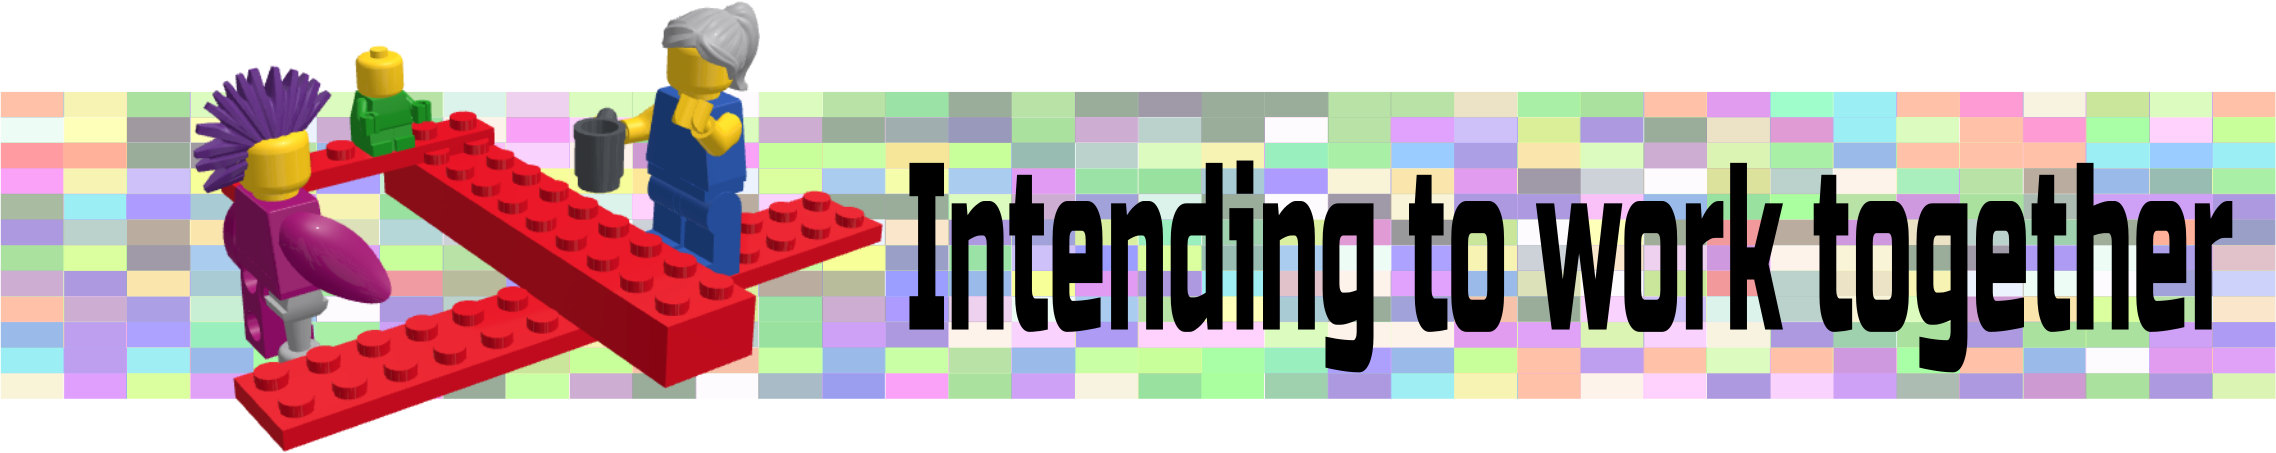
\includegraphics[width=\linewidth]{banner_Care_Big.png}
Leitlinien zum Umgang miteinander}
\newcommand\dos{\item[$+$]}
\newcommand\donts{\item[$-$]}


\date{\vspace{-10ex}}
%\date{}
%%\title{Leitlinien zum Miteinander auf der GPN}
\hypersetup{
  pdfkeywords={},
  pdfsubject={},
  pdfcreator={Emacs 24.5.1 (Org mode 8.2.10)}}
\begin{document}

\maketitle
Hallo und herzlich willkommen auf der Gulaschprogrammiernacht, einer
Veranstaltung mit Technik, leckerem Essen und vielen großartigen
Menschen. Die folgenden Tipps wollen ein Leitfaden zum Umgang mit
diesen sein, um zwischenmenschliche Probleme zu vermeiden und eine
tolle GPN für alle zu ermöglichen.



\section{Allgemeines}
\label{sec-1}
\begin{itemize}
\dos Behandle andere Leute möglichst so, wie sie behandelt werden
möchten. \dos Wenn du dir unsicher bist, frag höflich. \dos Wenn jemand
gemein ist, versucht, darüber zu reden. \dos Wenn es unangenehm wird,
oder du Hilfe brauchst, wende dich an unser CARE-Team (Chaos Awareness
Response Entropians). Wir tragen !!grüne Badges und sind unter der
Dectnummer 1234 erreichbar. Am Infotresen sind Fotos von uns.
\end{itemize}


\subsection{Erster Eindruck}
\label{sec-1-1}
Wow, ganz schön viele Leute hier...\\ \emph{Jep, alleine die
  Online-Anmeldungen lagen über 1000 und die GPN wächst
  weiter}\\\\ Sind das alles Nerds?\\ \emph{Manche wollen sich das
  ganze auch einfach nur anschauen. Vielleicht sind ein paar davon ja
  auch welche von uns und wissen es nur noch nicht ;-)}\\\\ OK, aber
was ist mit\ldots{}?}\\ \emph{Zu einigen Gruppen findest du im
    folgenden weitere Informationen. Read on.}


\section{Mädchen und Frauen}
\label{sec-2}
Wow, hier sind ja Mädels! Die sind doch bestimmt mit ihrem Freund da?
Und wenn nicht, kann ich sie anbaggern? Ich könnte nämlich ne Freundin
gebrauchen\ldots{}


\emph{Leider ist der Frauenanteil in technischen Berufen ziemlich
  gering. Viele empfinden das Umfeld als unangenehm und bleiben nicht
  lange dabei. Bitte sei nicht der Grund dafür.}

\label{sec-2-1}
\begin{itemize}
\dos Behandle Mädchen und Frauen mit Respekt und Höflichkeit. Viele davon
haben (auch im Chaos) schon miese Erfahrungen gemacht.
\dos Frag nach Projekten, Spaces und Interessen, genau wie sonst auch.
\label{sec-2-2}
\donts Dauernd angegraben werden kann echt nerven. Wenn die Situation
  nicht gerade eindeutig auf Flirten hinausläuft, lass es sein.
\donts Genauso schlimm: Ständig in die Mädchenrolle gedrängt zu
  werden. Der Klassiker: oder "Was machst denn DU hier?". Auf einer
  Chaosveranstaltung von Gleichgesinnten die Technikkompetenz
  abgesprochen zu bekommen frustriert viele junge Haecksen endlos.
%\item Anderesrum stresst es auch, ständig am männlichen Maßstab
%  gemessen zu werden und gefühlt nichts gegen eklige, verstörende
%  oder sexistische Sprüche  sagen zu dürfen, ohne den Status als cooles
%  Mädchen zu verlieren. Anstand und Höflichkeit helfen.
%\item Nicht jede von uns ist Feministin, Expertin für Frauenprobleme
 % oder eine Koryphäe des Sozialen. Es ist ätzend, sich für andere
 % Frauen rechtfertigen oder sie erklären zu müssen, und den modernen
  %Feminismus gegen wikipediaerfahrenen Rethoriker verteidigen zu
  %sollen. Wir sind zum Hacken und für nette Leute hier, lasst den
  %anderen Kram in Ruhe, außer wir zeigen deutliches Interesse daran.
\end{itemize}

\subsection{Wenn du selbst weiblich bist und Stress mit den Jungs hast}
Komm zu uns oder ruf uns an. Wir haben auch Mädels im Team und dulden
keinen Sexismus auf der GPN.


\section{Neurodivergente}
\label{sec-3}
Ein paar Leute hier sind \ldots{} irgendwie seltsam. Sie schauen
z.B. beim Reden weg, schnippen mit den Fingern oder wiegen sich hin
und her und scheinen das lustig zu finden. Irgendwie kommt bei
Gesprächen keine richtige Verbindung auf. Was ist da los?


\emph{Neurodivergenz ist bei weitem noch nicht vollständig
  erforscht. Viele Neurodivergente leiden darunter, dass Neurotypische
  (also Menschen die nicht neurodivergent sind) nicht mit ihnen
  klarkommen oder sie zwanghaft in Stereotypen pressen wollen. Dabei
  würde es auch neurotypischen Menschen helfen, sich mit dieser
  Andersartigkeit auseinander zu setzen und die eigenen Vorstellungen
  zu reflektieren}

\label{sec-3-1}
\begin{itemize}
\dos Auch Neurodivergente sind hier um Spaß am Gerät zu haben und
  nette Leute zu treffen. Behandle sie also so, dass sie sich als Teil
  des Ganzen fühlen können. Ohne Bevormundung.
\dos Freundliche Nachfragen werden oft bereitwillig beantwortet. Hier
  braucht es Fingerspitzengefühl.
\donts Niemand mag nur auf einen Aspekt reduziert werden. Lass den
  Leuten auch Raum, eine Person zu sein und reduziere sie nicht auf
  ihre Andersartigkeit. Akzeptiere, wenn sie wütend sind.
\donts Bestehe nicht darauf, dass sich alle Neurodivergente wie
  ``typische'' Autisten/Asperger verhalten, auch wenn du solche
  Menschen kennst.
\donts Diagnosen sind ganz dünnes Eis. Niemand braucht eine offizielle
  Diagnose um anders zu sein und oftmals wird durch das medizinische
  Establishment sehr viel Schaden angerichtet.
\end{itemize}

\subsection{Wenn du selbst neurodivergent bist und die Neurotypischen Probleme machen}
Komm zu uns oder ruf uns an, haben Erfahrung in dem
Bereich und können dir weiterhelfen.

\section{Trans* \& Queer}
\label{sec-5}
Hier sind Leute bei denen ich mir nicht sicher bin, ob sie Männchen
oder Weibchen sind. Und ein paar sehen eindeutig aus, tragen aber
diese Pronomenschilder und da steht was anderes drauf. Und ein paar
davon sind offensichtlich ineinander verliebt. Das ist alles nur Spaß,
oder?

\emph{Geschlecht und Begehren sind sozial konstruiert und werden
  zunehmend in Frage gestellt. Immer mehr Menschen leben als das
  andere, ein drittes, ganz ohne, oder mit wechselndem
  Geschlecht. Andere experimentieren mit diesen
  Ausdrucksformen. Außerdem verlieben sich alle möglichen Leute
  ineinander.}
\label{sec-5-1}
\begin{itemize}
\dos Respektiere Pronomen, Namen und Identitäten. Niemand ist
  verpflichtet dir irgendwas zu beweisen. Frag am besten voher welches
  Prononem passt, statt nur zu schätzen. Auch der Name kann hier ein
  deutlicher Hinweis sein. Wenn du damit absolut nicht klarkommst,
  lass diese Leute in Ruhe und denk in Ruhe drüber nach.
\dos Ähnliches gilt für andere Sexualitäten: Wenn du nicht auf
  jemanden stehst, sag das und versuche umgekehrt nicht, Leute zu
  ``bekehren''.
\donts Erschlage Leute nicht mit Stereotypen. Das Fernsehen
  lügt. Youtube auch.
\donts Bitte erkläre Leuten nicht, auf welche Toiletten sie gehen oder
  nicht gehen können. Falls es hier zu irgendwelchen Problem kommt
  (wie z.B. Kerlen die solche Vorgaben missbrauchen um Mädchen und Frauen
  zu belästigen), hol uns oder die Orga.
\end{itemize}
\subsection{Wenn du selbst trans* oder queer bist}
Melde dich bei uns, falls irgendwas ist, wir helfen dir weiter. Wenn
du Fragen hast oder einfach nur mit jemandem reden magst, der dich
versteht, wende dich an unsere queere Nonbinäre, Lisa.




\section{People of Color (PoC), Menschen mit
  Migrationshintergrund}
\label{sec-4}
Da sind Leute, die aussehen als ob sie von weit weg herkämen. Soll ich
ihnen Deutschland erklären?

\emph{Technikbegeisterung ist ein weltweites Phänomen. Wer (egal
  woher) auf die GPN kommt, will wahrscheinlich vor allem freundliche
  Menschen treffen und mit spannender Technik spielen.
  Kosmopolitismus rockt.}
\label{sec-4-2}
\begin{itemize}
\dos Hilf Leuten gegebenenfalls beim Übersetzen. Im Zweifel sind
  klare Aussagen besser als grammatikalisch elaboriertes Englisch.
\donts Stereotype (auch vermeintlich positive) können sehr schmerzhaft
  sein. Sei dir dessen bewusst und lass Leute damit in Ruhe.
\donts Bitte fass Leuten nicht ungefragt an. Auch nicht, wenn sie eine
  spannende Frisur haben.
\end{itemize}
\subsection{Wenn du einen Migrationshintergrund hast oder POC bist und Hilfe brauchst / If you are a POC or a migrant and want help}
Ruf uns einfach an, wir helfen dir. Just give us a call, we will help
you.


\section{Kinder}
\label{sec-6}
 Wow hier sind ja wirklich kleine Menschen. Haben die sich verlaufen?

 \emph{Die GPN zieht Menschen aller Altersklassen an. Außerdem
  versuchen diverse Initiativen wie z.B. ``Chaos macht Schule'' auch
  dem Nachwuchs vernünftige Medienkompetenz zu vermitteln.}


\label{sec-6-1}
\begin{itemize}
\dos Du bist älter, sei ein Vorbild.
%\item Wenn sich die Kleinen für dein Projekt interessieren, erklär
%  es. Benutz dafür altersangemessene Begriffe und wiederhole wichtige
%  Informationen. Mach dir nix draus, wenn die Kids trotzdem
%  weiterziehen.
\dos Versuch dich zu erinnern. Was würdest du dir als Kind in der
  Situation von den Großen wünschen, was davon wäre sinnvoll? Sei
  diese Person.
\donts Bitte sei nicht fies. Wenn du Ruhe brauchst, sag das
  freundlich. Auch Kinder haben Gefühle.
\donts Bitte streite dich nicht mit den Kleinen. Ruf lieber uns, wir klären
das.
\end{itemize}
\subsection{Wenn du selbst noch jung bist und irgendwelche Hilfe brauchst}
Komm zu uns oder ruf uns auf einem Dectphone an. 


\section{Behinderungen}
Ok, ich glaub ich habs verstanden. Ich soll auf Menschen mit
Einschränkungen wie Stottern, Mobilitätseinschränkungen oder geistigen
Behinderungen besondere Rücksicht nehmen, ohne sie zu bevormunden,
stimmt's oder hab ich Recht?

\emph{Yay, du hast es kapiert.}


\label{sec-7-1}
\begin{itemize}
\dos Sei freundlich und hilf Leuten gegebenenfalls. Ruft uns an, wenn
  ihr Hilfe von der Orga braucht oder irgendwas unzugänglich ist.
\donts Sei nicht gönnerhaft, fall Leuten nicht ins Wort
  wenn sie einen Moment länger brauchen um etwas auszudrücken.
\donts Bitte verschieb nicht einfach Leute, egal ob im Rollstuhl oder
  ohne.
\end{itemize}



\section{Diese Regeln nerven! Ich glaube ich werde euch hart trollen müssen. Am besten ich bastle eine gigantische fliegende Vu\ldots}
\label{sec-8}
\ldots vuzela? Och, bitte nicht, das nervt doch. Ganz ernsthaft: Wir
finden es auch schade, dass wir überhaupt Leitlinien brauchen, aber
leider gibt es zu viele neue Leute um sich auf einen allgemeinen
Hackerkonsens zu berufen. Daher machen wir die Regeln vorher
explizit. Wenn du mit uns darüber streiten magst, besuch uns oder ruf
uns an. Am besten fragst du nach Lisa, die hat auch diesen Flyer
verbrochen.

\section{Das Careteam}
Du findest Fotos von uns auf dem Infodesk. Unsere Dectnummer ist
1234. Wir tragen grüne Badges. Im Zweifel frag einfach irgendwen vom
Entropia nach uns.



\end{document}
